\subsubsection{Triangulation}

\begin{frame}\frametitle{Cycles and chords}

\slidesonly{\vspace{-3mm}}

\begin{figure}[h]
\centering
	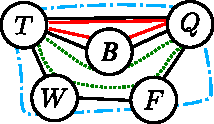
\includegraphics[height=2.cm]{img/cycles2}
	\mode<article>{
	\caption{Identifying cycles in an undirected graph}
	}
\end{figure}

\slidesonly{\vspace{-3mm}}

\begin{itemize}
\item \emph{Cycle}: A closed path with \textbf{no} repeated vertices \slidesonly{except}\notesonly{other than} $V_{\text{start}}=V_{\text{end}}$.
\item \emph{Chords}: Given a cycle, an edge is a chord if it connects two nodes that are non-adjacent on the cycle.
\item \emph{Chordless} cycle: \textbf{All} two \textbf{non}-adjacent vertices on the cycle are \textbf{not} joined by any edge.
\item \emph{Triangulated graph} ($\corresponds$ \emph{Chordal graph}): A graph \textbf{without} chordless cycles of 4+ vertices.\notesonly{\footnote{cf: Definition 2.24 on Ch. 2.2.4 in \citep{koller2009probabilistic}
%\citep{Jebaraslides}
}
}
\begin{flushright}
{\footnotesize(too many double negatives!!!)}
\end{flushright}
\end{itemize}

\slidesonly{\vspace{-2mm}}

\begin{block}{Triangulation}
Construct a chordal graph by adding \emph{chords} (``shortcut'' edges) to all cycles of length 4+.
\end{block} 

\end{frame}

%\newpage

\subsubsection{Triangulation: Examples}

\begin{frame}{Only} \frametitle{\subsubsecname}

\mode<presentation>{
\begin{block}{Triangulation}
Construct a chordal graph by adding \emph{chords} (``shortcut'' edges) all cycles of length 4+.
\end{block} 
}

\begin{enumerate}
\item<only@1>[]

	Consider the following graph with vertices $A,B,C,E$ \notesonly{in \figref{fig:triangulateexample1} }and add chords where necessary:
	\slidesonly{\textbf{(see blackboard)}}


	\begin{figure}[h]
	\centering
	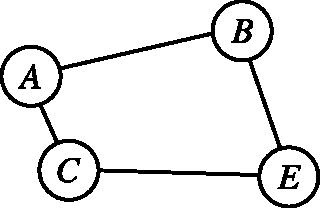
\includegraphics[height=2.5cm]{img/graph_example_triangulate}
	\caption{a non-decomposable graph}
	\label{fig:triangulateexample1}
	\end{figure}

\mode<article>{
		\begin{figure}[h]
		 \centering
		 \savebox{\imagebox}{
		 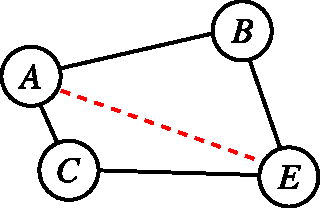
\includegraphics[width=0.2\textwidth]{img/graph_example_triangulate_sol1}}%
		 \begin{subfigure}[t]{0.25\textwidth}
			 \centering
			 \usebox{\imagebox}% Place largest image
			 %\caption{...}
		 \end{subfigure}
		 \hspace{7mm}
		 \begin{subfigure}[t]{0.2\textwidth}
			 \centering
			 \raisebox{\dimexpr.5\ht\imagebox-.5\height}{% Raise smaller image into place
			 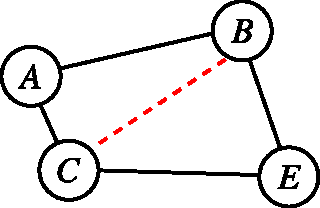
\includegraphics[width=0.99\textwidth]{img/graph_example_triangulate_sol2}
			 }
			 %\caption{...}%
		 \end{subfigure}
		 \caption{Possible triangulations for graph in \figref{fig:triangulateexample1}}
		\end{figure}
}


\item<only@2,3>[]

	Consider the following graph with vertices $A,B,C,W,E,F$ \notesonly{in \figref{fig:triangulateexample2} } and add chords where necessary:\\
	\slidesonly{\textbf{(see blackboard)}}


		\begin{figure}[h]
		 \centering
		 \savebox{\imagebox}{
		 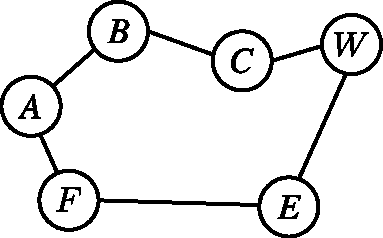
\includegraphics[width=0.25\textwidth]{img/graph_example2_triangulate}}%
		 \begin{subfigure}[t]{0.25\textwidth}
			 \centering
			 \usebox{\imagebox}% Place largest image
			 \caption{example graph to triangulate}
		 \end{subfigure}
		 \hspace{7mm}
		 \visible<3>{
		 \begin{subfigure}[t]{0.25\textwidth}
			 \centering
			 \raisebox{\dimexpr.5\ht\imagebox-.5\height}{% Raise smaller image into place
			 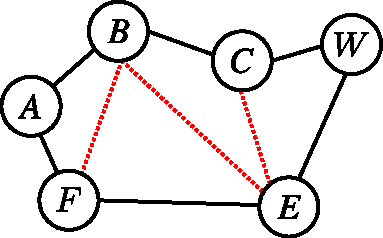
\includegraphics[width=0.99\textwidth]{img/graph_example2_triangulate_sol1}
			 }
			 \caption{One possible and non-unique triangulation}%
		 \end{subfigure}
		 \caption{Triangulation example}
		 \label{fig:triangulateexample2}
		 }
		\end{figure}

\item<only@4,5>[]

	\question{Is this a chordal graph\notesonly{ (c.f. \figref{fig:triangulateexample3})}? i.e. does it contain chordless cycles with 4+ vertices?}\\


		\begin{figure}[h]
		 \centering
		 \savebox{\imagebox}{
		 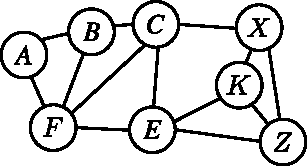
\includegraphics[width=0.3\textwidth]{img/graph_example3_triangulate}}%
		 \begin{subfigure}[t]{0.35\textwidth}
			 \centering
			 \usebox{\imagebox}% Place largest image
			 \caption{example graph}
		 \end{subfigure}
		 \hspace{5mm}
		 \visible<5>{
		 \begin{subfigure}[t]{0.3\textwidth}
			 \centering
			 \raisebox{\dimexpr.5\ht\imagebox-.5\height}{% Raise smaller image into place
			 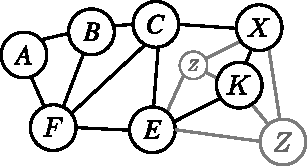
\includegraphics[width=0.99\textwidth]{img/graph_example3_triangulate_HINT}
			 }
		 \mode<article>{
			 \caption{The cycles CEKX and CEZX both require chords for the graph to be chordal.}%
			 }
		 \end{subfigure}
		 \mode<article>{
		 \caption{Determining if a graph is chordal}%
		 }
		 \label{fig:triangulateexample3}
		 }
		\end{figure}
		
\end{enumerate}

\end{frame}
